\section{Grundlegende Architektur des Testmodells}
\label{sec:modelArchitecture}

Um Hadoop mit der Selfbalancing"=Komponente mit den in \cref{sec:requirements} beschriebenen Anforderungen prüfen zu können, wird mithilfe des \gls{ss}"=Frameworks ein vereinfachtes Modell der relevanten YARN"=Komponenten entwickelt.
Dieses YARN"=Modell wird mithilfe des Treibers mit dem realen Cluster verbunden, was durch hierfür entwickelte Scripte gesteuert wird.
Daraus resultiert folgende Drei"=Schichten"=Architektur für das gesamte Testmodell:

\begin{figure}[h]
    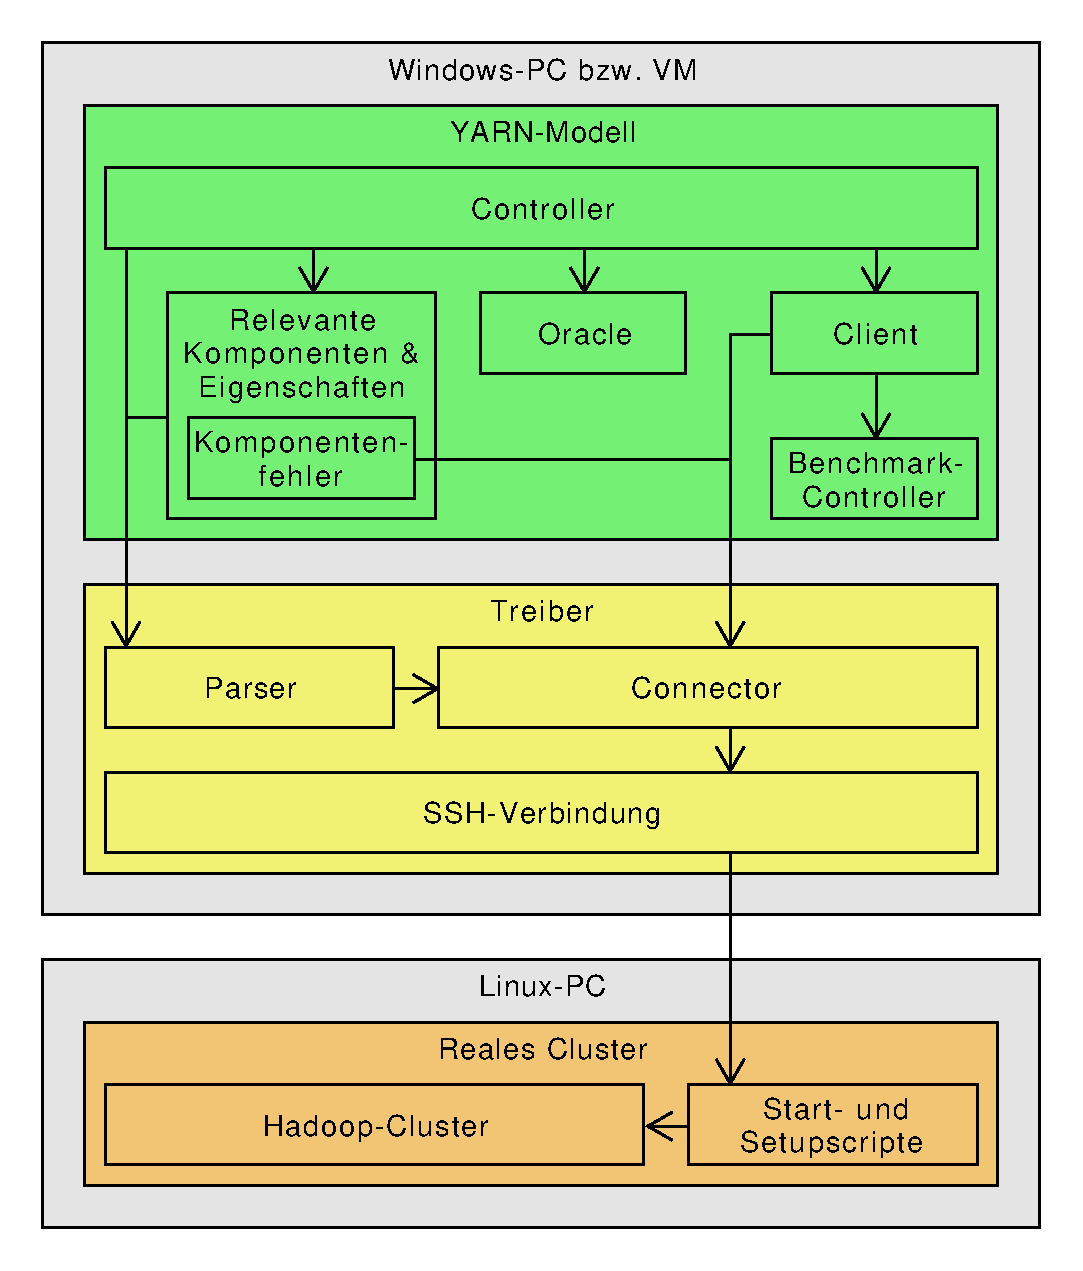
\includegraphics[width=0.6\columnwidth]{./resources/modelArchitecture.pdf}
    \caption{Grundlegende Architektur des Testmodells}
    \label{fig:modelArchitecture}
\end{figure}

Das YARN"=Modell stellt die oberste Schicht des Testmodells dar.
Es bildet das Kernstück dieser Fallstudie, da dieses Modell mit den hierin abgebildeten YARN"=Komponenten und Komponentenfehlern, dem Controller und dem Oracle direkt im Rahmen des modellbasierten Testens mit \gls{ss} interagiert.
Folgende Komponenten sind im YARN"=Modell enthalten:

\begin{description}
    \item [Controller] \hfill \\
        Steuert den Ablauf einer Testausführung und das Zusammenspiel zwischen den Komponenten des YARN"=Modells.
    \item [Relevante YARN"=Komponenten und Eigenschaften] \hfill \\
        Bilden die grundlegende Architektur von Hadoop YARN ab.
        Implementiert wurden in dieser Fallstudie die Nodes, Anwendungen, Attempts und Container mit den jeweils relevanten Eigenschaften zur Durchführung der Fallstudie.
    \item [Komponentenfehler der YARN"=Komponenten] \hfill \\
        Bilden die bei den Tests zu injizierenden Komponentenfehler der jeweiligen YARN"=Komponenten.
    \item [Oracle] \hfill \\
        Validiert die in Form von Constraints in den jeweiligen YARN"=Komponenten implementierten Anforderungen.
    \item [Client] \hfill \\
        Dient zum starten und beenden von Benchmarks im Cluster.
    \item [Benchmark"=Controller] \hfill \\
        Enthält das Transitionssystem zur Auswahl der Benchmarks und steuert diese.
\end{description}

Die Verbindung zwischen dem YARN"=Modell und dem realem Cluster bildet der Treiber.
Er besteht aus folgenden Komponenten:

\begin{description}
    \item [Parser] \hfill \\
        Verarbeitet die Monitoring"=Ausgaben vom realen Cluster und konvertiert diese für die Nutzung im YARN"=Modell.
    \item [Connector] \hfill \\
        Abstrahiert die Verbindung zum realen Cluster und die dabei auszuführenden Befehle.
    \item [SSH"=Verbindung]  \hfill \\
        Stellt die Verbindung zum realen Cluster her.
\end{description}

Der Parser wird hierbei nur zur Durchführung des Monitoring benötigt und nutzt wiederum den Connector zum abrufen der Daten.
Andere Befehle und Zugriffe auf das reale Cluster, wie \zB das Injizieren von Komponentenfehlern, werden direkt mithilfe des Connectors durchgeführt.

Alle Informationen des Monitorings, der Validierung der Constraints oder Debug"=Informationen werden während der Ausführung im Programmlog gespeichert (vgl. \cref{subsec:yarnComponentInterface,subsec:oracleImpl}).
Zu Analysezwecken im Fehlerfall wird zudem jede Kommunikation der SSH"=Verbindungen in einem eigenen Log, dem SSH"=Log, abgespeichert (vgl. \cref{subsec:sshConnection}).
Durchgeführt wird dies mithilfe des Frameworks log4net\footnote{\url{https://logging.apache.org/log4net/}}, mit denen an den entsprechenden Stellen im Programm das Logging durchgeführt wird.

Die Implementierung des YARN"=Modells wird in \cref{sec:yarnModel,sec:benchmarkController} beschrieben, die Implementierung des Treibers in \cref{sec:sshDriver}.
Die Umsetzung des realen Clusters wird in \cref{sec:realCluster} beschrieben.
